\documentclass{beamer}

\usetheme{Berlin}
\usefonttheme{structurebold}

\title{The Mirai Botnet}
\author{Ulysses Butler, Thu Vo, and Tung Thai, Torey Clark}

\institute{ Truman State University \\ Binary Beasts }

\date{}

\begin{document}

\maketitle

\section{Introduction}

\begin{frame}
	\frametitle{The Paper}
	\begin{itemize}
		\item<+-> Title: \textit{Understanding the Mirai Botnet}
		\item<+-> \textit{The Proceedings of the 26th USENIX Security Symposium}
		\item<+-> This paper explores the Mirai botnet
		\item<+-> This botnet was responsible for one of the largest DDoS attacks every recorded.
		\item<+-> The researchers reverse engineer binaries used by the botnet to determine how it worked, how it spread, and what damage it did
	\end{itemize}
\end{frame}

\section{Spreading Mirai}

\begin{frame}
	\frametitle{Bootstraping}
	\begin{itemize}
		\item<+-> August 1, 2016: Servers owned by DataWagon began a preliminary scan.
		\begin{itemize}
			\item<+-> DataWagon is a bulletproof web hosting provider.
			\item<+-> Users are allowed to upload to upload and distribute almost anything using their service.
		\end{itemize}
		\item<+-> After this scan, the botnet started infecting computers
		\begin{itemize}
			\item<+-> 1 minute -  800 infected devices
			\item<+-> 10 minutes - 11,000 infected devices
			\item<+-> 20 hours - 65,000 infected devices
			\item<+-> Held steady at around 100,000 to 200,000 infections
			\item<+-> In December 2016, it peaked at 600,000 devices before beginning to fade
		\end{itemize}
	\end{itemize}
\end{frame}

\begin{frame}
	\frametitle{Spreading}
	\begin{columns}
		\column{0.5\linewidth}
			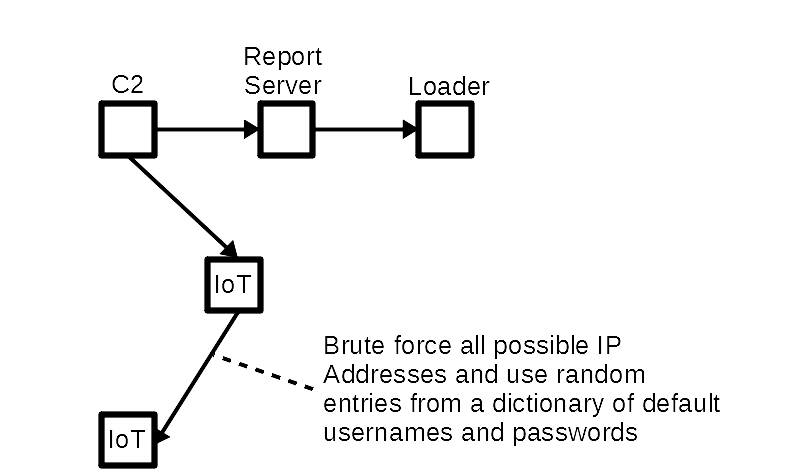
\includegraphics[width=\textwidth]{fig1.png}
		\column{0.5\linewidth}
			\begin{itemize}
				\item<+-> A member of the botnet begins scanning scanning ports on all IPv4 addresses
				\item<+-> It scans to find open ports for SSH, Telnet, FTP, and other protocols
				\item<+-> It would then use a dictionary attack to brute force into the machine
				\item<+-> These were small dictionaries, containing 60 to about 200 credentials
			\end{itemize}
	\end{columns}
\end{frame}

\begin{frame}
	\frametitle{Spreading}
	\begin{columns}
		\column{0.5\linewidth}
			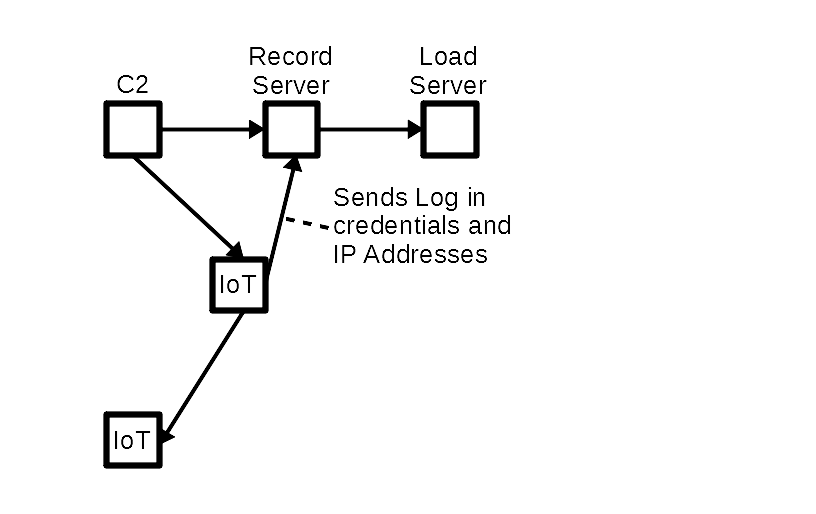
\includegraphics[width=\textwidth]{fig2.png}
		\column{0.5\linewidth}
			\begin{itemize}
				\item<+-> The address and credentials of the victim machines where then sent to a report server
				\item<+-> This information could later be used by the Command and Control (C2) server
			\end{itemize}
	\end{columns}
\end{frame}

\begin{frame}
	\frametitle{Spreading}
	\begin{columns}
		\column{0.5\linewidth}
			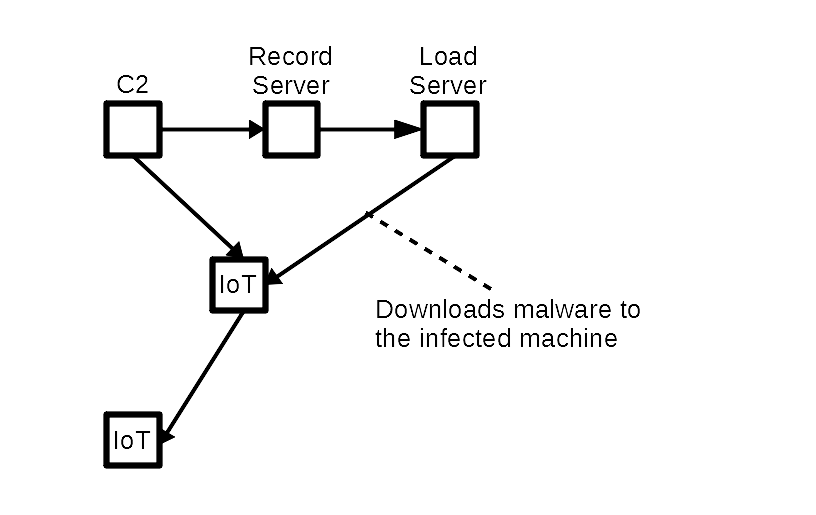
\includegraphics[width=\textwidth]{fig3.png}
		\column{0.5\linewidth}
			\begin{itemize}
				\item<+-> The records server then sent this information to the load program
				\item<+-> This program would download a binary onto the victim and run the program
			\end{itemize}
	\end{columns}
\end{frame}

\begin{frame}
	\frametitle{Loading the Binary}
	\begin{itemize}
		\item<+-> The aforementioned loader program downloaded an architecture specific binary
		\item<+-> The machine would then run the binary and change the process information to make it harder to detect
		\item<+-> The binary is then deleted.
		\begin{itemize}
			\item<+-> This means infections won't carry across reboots
		\end{itemize}
		\item<+-> Once the victim is infected, it starts scanning
		\begin{itemize}
			\item<+-> It would specifically avoid scanning servers owned by major corporations or the government
			\item<+-> These entities would likely be too secure for this simple attack
			\item<+-> This also allowed the bot to keep a lower profile
			\item<+-> These organizations would be much more likely to start search for and exploiting weaknesses in the malware if it infected their machines
		\end{itemize}
	\end{itemize}
\end{frame}

\section{Exploiting IoT Devices}

\begin{frame}[fragile]
	\frametitle{Internet of Things Security}
	\begin{itemize}
		\item<+-> The Internet of Things
		\begin{itemize}
			\item<+-> Includes security cameras, routers, network-access storage, TV receivers, etc.
			\item<+-> Typically embedded systems that aren't powerful
		\end{itemize}
		\item<+-> Manufactures neglect security
		\begin{itemize}
			\item<+-> Many manufactures use one user name and password
			\item<+-> Common passwords are frequent. \verb|password|, \verb|admin|, etc.
			\item<+-> Some devices even have credentials hard coded in firmware
			\item<+-> Most companies don't have the infrastructure to release patches for these systems
		\end{itemize}
		\item<+-> This allowed the bot to easily infect a large number of machines
	\end{itemize}
\end{frame}

\begin{frame}
	\frametitle{Disadvantages}
	\begin{itemize}
		\item<+-> These less powerful devices also hurt Mirai's growth
		\begin{itemize}
			\item<+-> Mirai had a doubling time of 75-minutes
			\begin{itemize}
				\item<+-> Compare to 37-minutes for Code-Red
				\item<+-> 9-minutes for Blaster
			\end{itemize}
			\item<+-> Most bots scanned at less than 250 bytes per second
			\item<+-> Much slower than other bot nets
			\item<+-> SQL Slammer was about 6000 times faster at 1.5 megabytes per second
		\end{itemize}
		\item<+-> Most devices were found in low bandwidth countries
		\begin{itemize}
			\item<+-> Most infected devices were from South America and South-east Asia
			\item<+-> Brazil, Colombia, and Vietnam hosted most of the bots
		\end{itemize}
	\end{itemize}
\end{frame}

\section{Attacking}

\begin{frame}{Attacks}
	\begin{itemize}
		\item<+->Distributed Denial of Service (DDoS) Strategies
			\begin{itemize}
				\item<+->Multiple DDoS attacks against a variety of targets
				\item<+->Game Servers (primarily Minecraft and Runescape)
				\item<+->Political Websites, anti-DDoS protectors
			\end{itemize}
		\item<+->Notable Targets
			\begin{itemize}
				\item<+->Krebs on Security - largest reported DDos attack to that point
				\item<+->Dyn - DNS attack disrupted access for Amazon, Github, Netflix, Twitter, and others
				\item<+->Lonestar Cell - most attacked target, destroyed internet capabilities in Liberia
			\end{itemize}
	\end{itemize}
\end{frame}

\section{Open Source Software}

\begin{frame}
	\frametitle{Releasing the Source Code}
	\begin{itemize}
		\item<+-> The source code was released on September 30, 2016
		\item<+-> A user named ``Anna-senpai'' released the source code for free on hackerforums.net
		\item<+-> This spawned a number of copycat attacks with variations on the original bot
		\begin{itemize}
			\item<+-> Many included new exploits, modified dictionaries, and different IP blacklists
		\end{itemize}
		\item<+-> These botnets eventually starting competing
		\begin{itemize}
			\item<+-> Killing processes started by similar bots
			\item<+-> Closing the ports used to attack the machine
			\item<+-> At various points, competing command and control servers were subject to DDoS attacks
		\end{itemize}
	\end{itemize}
\end{frame}

\section{Defending Against Mirai}

\end{document}
